%% -*- mode: latex; mode: flyspell -*-
\documentclass[12pt, letter]{article}

%% Class name and Assignment number
%%
\newcommand{\courseName}{ECE 435 Medical~Image~Processing}
\newcommand{\assignName}{Assignment~4}

%% Packages
\usepackage{amsmath,amsfonts,amssymb,amsthm,dsfont}
\usepackage{graphicx}
\usepackage[bookmarks=false]{hyperref}
\usepackage{color}
\usepackage{lipsum}
\usepackage{amsmath}
\usepackage{booktabs}
\usepackage{subfig}
%% Paper format
\usepackage{geometry}
\geometry{
    letterpaper,
    %% total={216mm,279mm}, %< NSERC size
    margin=2.00cm,     %< default
    %% margin=1.87cm,       %< NSERC tightest
}

%% Headers and footers
\usepackage[explicit]{titlesec}
\newpagestyle{titlesec_assignment}{
  \sethead{\courseName}{}{\assignName}\setfoot{}{\thepage}{}
  \headrule
  %% \footrule
}

\begin{document}

%% Set header and footer
\pagestyle{titlesec_assignment}

%% Title
\title{\courseName\\\assignName}
\author{Yiping Wang V00894385}
\maketitle

\paragraph{Question 1: } Implement the algorithm on Basic Global Thresholding described in L8.1. The implementation of your algorithm needs to specify a tolerance percentage below which the thresholds T(i+1) and T(i) are considered identical. This tolerance parameter needs to be an input for your function.

\paragraph{Answer: } Please see the ``basic\_global\_thresholding.m'' inside this folder. 


\paragraph{Question 2:} Test the algorithm on the image ``angiogram.tif''. You will provide the following results:
\begin{enumerate}
    \item The binarized image with the value of the threshold at convergence
    \item The histogram of ‘angiogram.tif’ image with the value of the threshold specified on it.
    \item A table containing the value of the threshold at every iteration before reaching convergence.
\end{enumerate}

\paragraph{Answer:}
The following results are obtained when tolerance is set to $\mathbf{10^{-8}}$. The initial estimate of the threshold is randomly selected from the element of the image.  

The binarized image with threshold at convergence of $\mathbf{103.9122}$, the histogram of ``angiogram.tif'' image with the threshold at convergence of $\mathbf{103.9122}$ and the histogram of number of binary values are shown in Figure~\ref{fig:q2-1}. Table~1 shows the value of the threshold at every iteration before reaching convergence.

\begin{figure}
    \centering
    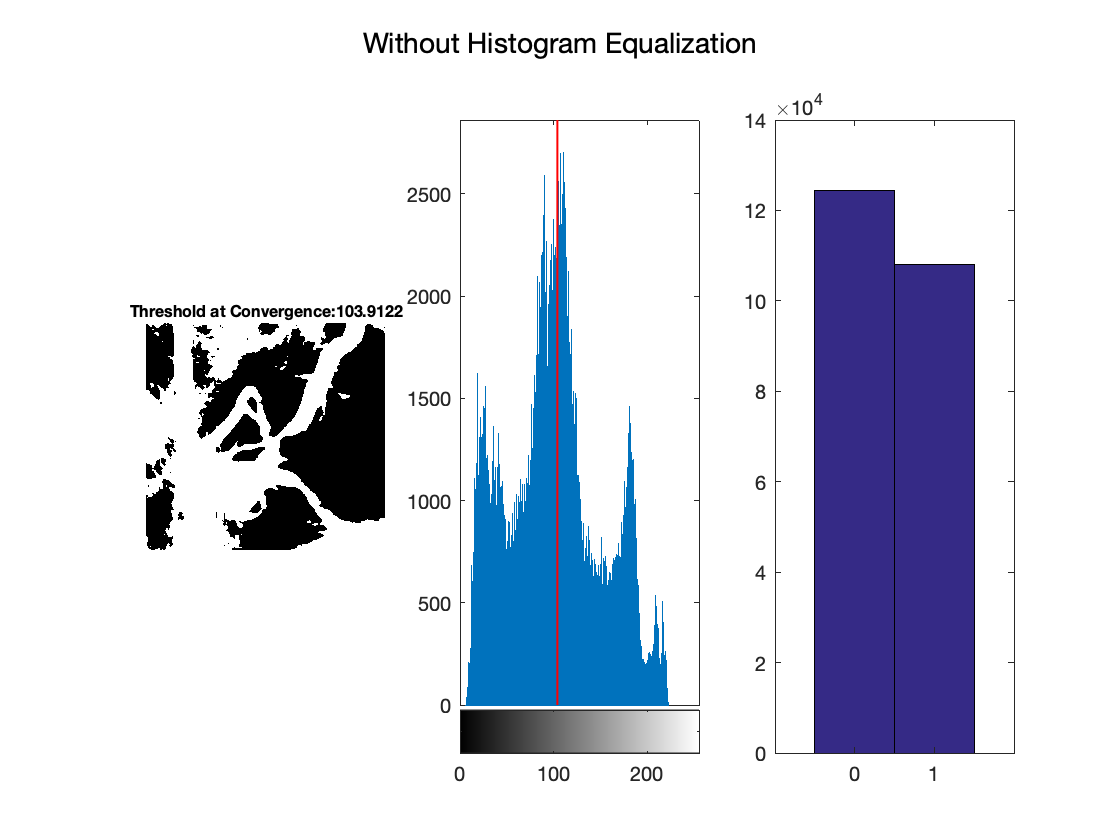
\includegraphics[width=14cm]{without-histogram-equalization.png}
    \caption{(a) Binarized Image; (b)  ``angiogram.tif'' Image Histogram; Red Line Marks the Threshold at Convergence of 103.9122; (c) Histogram of Number of Binary Values}
    \label{fig:q2-1}
\end{figure}

\begin{center}
\begin{tabular}{llr}  
\toprule
\multicolumn{2}{c}{Table 1} \\
\cmidrule(r){1-2}
Iteration   & Threshold Value \\
\midrule
1      & 89 \\
2 & 93.4788 \\
3  & 96.4683 \\
4     & 98.5574 \\
5 & 100.0893 \\
6 & 101.6115 \\
7 & 102.3741 \\
8 & 103.1515 \\
9 & 103.9122 \\
\bottomrule
\label{table:q2-1}
\end{tabular}    
\end{center}

Since the initial estimate of the threshold is randomly selected from the element of the image, the result of converage could be different. 

\paragraph{Question 3:} Apply histogram equalization to ``angiogram.tif''. You may choose to work with the Matlab \textbf{histeq} function. Next, apply the same thresholding algorithm to the equalized image. Compute the new threshold, and the new binarized images

\paragraph{Answer:} The following results are obtained when tolerance is set to $\mathbf{10^{-8}}$. The initial estimate of the threshold is randomly selected from the element of the image.  

The binarized image with threshold at convergence of $\mathbf{127.0794}$ and the histogram of ``angiogram.tif'' image with the threshold at convergence of $\mathbf{127.0794}$ shows in Figure~\ref{fig:q3-1}. Table~2 shows the value of the threshold at every iteration before reaching convergence.

\begin{figure}
    \centering
    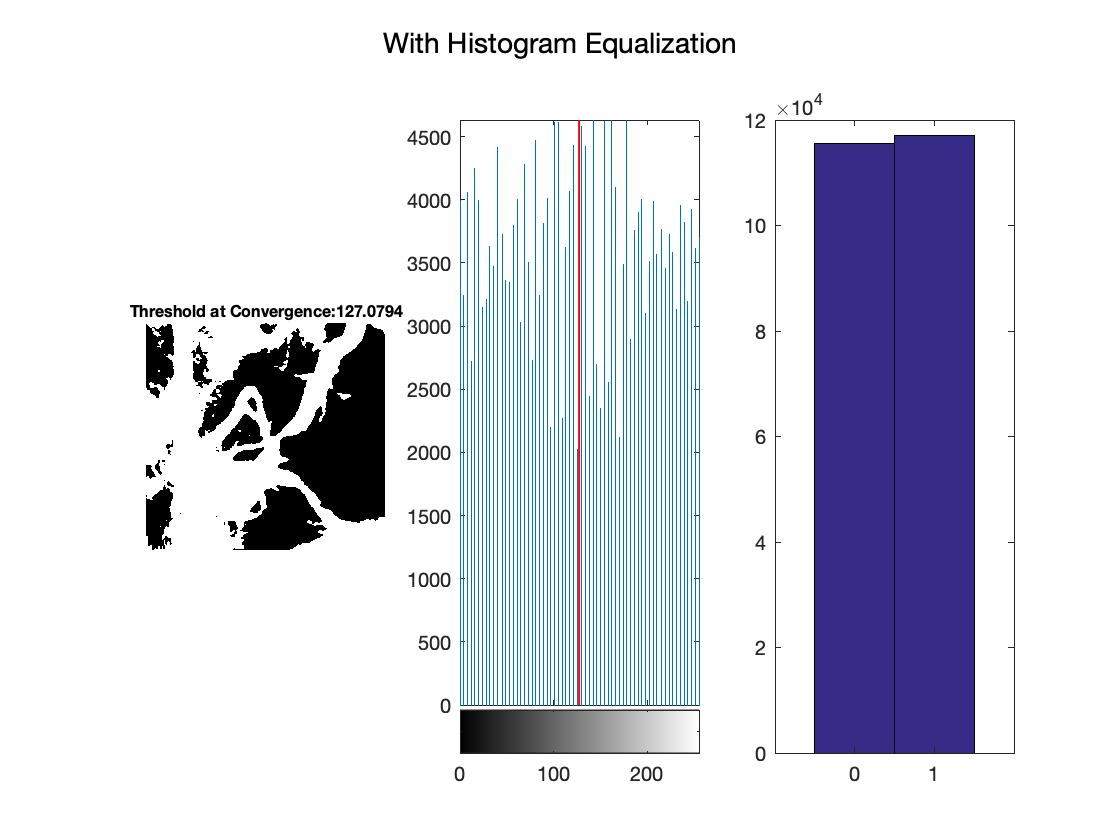
\includegraphics[width=14cm]{with-histogram-equalization.png}
    \caption{(a) Binarized Image; (b) ``angiogram.tif'' Image Histogram; Red Line Marks the Threshold at Convergence of 127.0794; (c) Histogram of Number of Binary Values}
    \label{fig:q3-1}
\end{figure}

\begin{center}
\begin{tabular}{llr}  
\toprule
\multicolumn{2}{c}{Table 2} \\
\cmidrule(r){1-2}
Iteration   & Threshold Value \\
\midrule
1 & 28 \\
2 & 78.6122 \\
3 & 102.8717 \\
4 & 115.3512 \\
5 & 121.2035 \\
6 & 125.9473 \\
7 & 127.0794 \\

\bottomrule
\label{table:q2-2}
\end{tabular}    
\end{center}

Since we pre-process the image using the Histogram Equalizationtion, the threshould of converage always converages to the same number, unlike the case without Histogram Equalization. Moreover, we can observe that the two bins of the binary values in the histogram (Figure~\ref{fig:q3-1} (c)) are roughly the same. 

\paragraph{Question 4: } Compare and discuss the results obtained by optimal thresholding on the original image, and on the image pre-processed with histogram equalization.

\paragraph{Answer: }

The optimal thresholding on without and with histogram equalization of ``angiogram.tif'' are shown in Figure~\ref{fig:com}. 

The Ostu's Method assumes that the image contains two classes of pixels following bi-modal histogram, it then calculates the optimum threshold separating the two classes so that their within-group variance is minimal. The Histogram Equalization is used to enhance contrast.

Without Histogram Equalization, the global threshold using Otsu's method is $\mathbf{0.4157}$. With Histogram Equalization, the global threshold using Otsu's method is $\mathbf{0.4980}$, which is very close to 0.50. From 
Figure~\ref{fig:com} (b), we can observe the white area is larger than Figure~\ref{fig:com} (a), especially in the left region since the Histogram Equalization attempts to balance the distribution of the gray values inside the image. Moreover, from Figure~\ref{fig:q2-1} or Figure~\ref{fig:q3-1}, we know the histogram of input image is not a bi-model histogram, which explains why the Ostu's Method does not perform very well in this specific image.

\begin{figure}%
	\centering
	\subfloat[Without Histogram Equalization]{{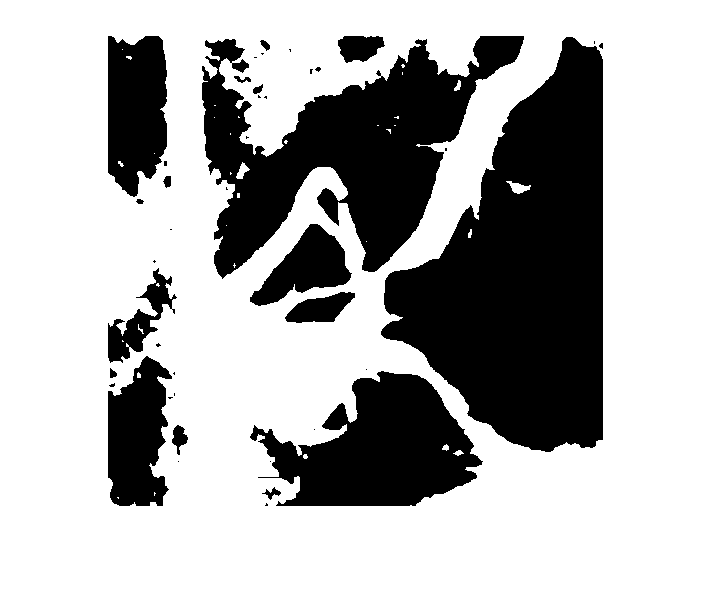
\includegraphics[width=7cm]{ostu-without-hist-equ.png}} }%
	\qquad
	\subfloat[With Histogram Equalization]{{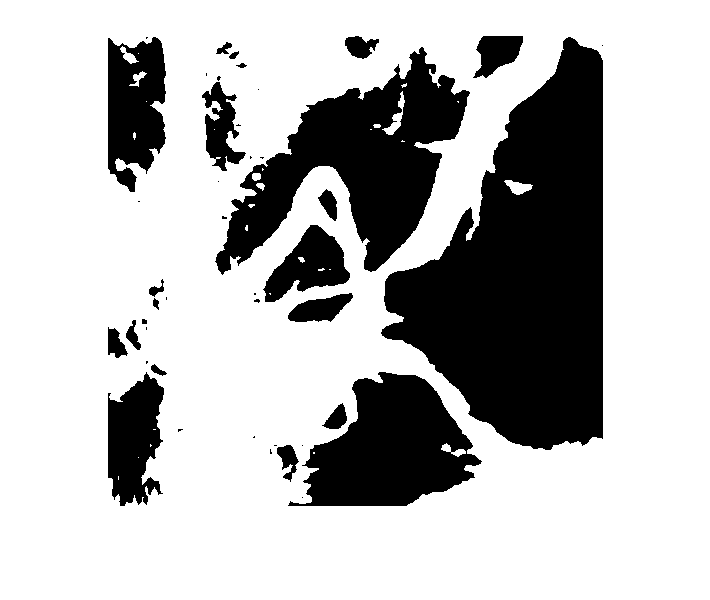
\includegraphics[width=7cm]{ostu-with-hist-equ.png}} }%
	\caption{Results of Optiomal Thresholding Without and With Histogram Equalization}%
	\label{fig:com}%
\end{figure}

\end{document}


%%% Local Variables:
%%% mode: latex
%%% TeX-master: t
%%% End:
